\chapter{Technologien für Windows Desktop-Anwendungen}
\label{chap:TechnologienfürWindowsDesktop-Anwendungen}

\section{Notification Area}
Als Notification Area werden alle rechtsbündigen Symbole bis zu dem Pfeil, der nach oben zeigt bezeichnet, wenn man auf den Pfeil klickt wird die Overflow Area geöffnet. In diesen Bereich werden standardmäßig einige Symbole verschoben. Jedes Symbol kann von der Notification Area in die Overflow Area verschoben werden dasselbe gilt auch für die andere Richtung.\footnote[1]{\cite[Vgl.][]{10}}
\begin{figure}[H]
    \centering
    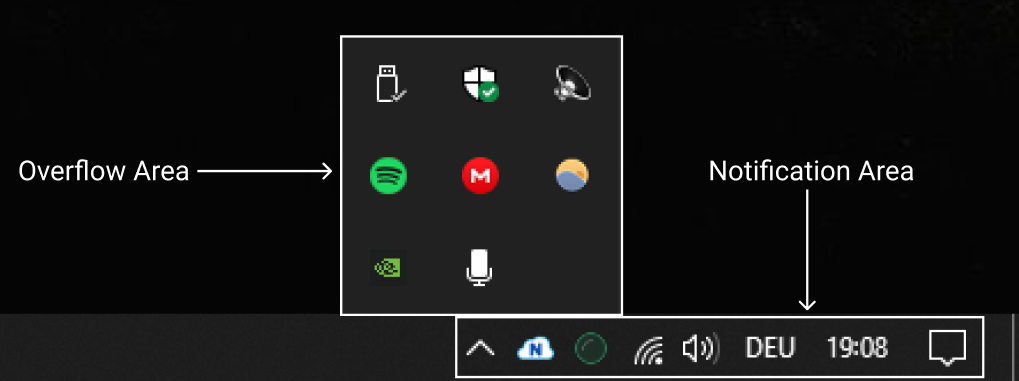
\includegraphics[width=0.8\textwidth]{NotificationArea.png}
    \caption[NotificationArea]{Notification Area} 
\end{figure}

\newpage
\ \\
Die Notification Area ist besser bekannt unter dem Namen Systemtray, wird aber offiziell von Windows als Notification Area bezeichnet. Der Begriff Systemtray kommt von Windows 95, weil es da eine Anwendung gibt die systray.exe heißt. Nachdem dieses Programm geschlossen wurde, sind die Symbole die in der Notification Area angezeigt wurden verschwunden. Deshalb hat man angenommen, da die Anwendung die dafür zuständig ist systray.exe heißt. Der Name des Bereichs wo die Symbole angezeigt werden Systemtray ist. Das ist aber nicht der einzige Grund der Verwirrung gewesen. Microsoft Mitarbeiter haben den Bereich als Systemtray bezeichnet und bis 2003 war auch in der Windows Dokumentation der Begriff Systemtray enthalten. Nicht nur in der Dokumentation ist Windows so ungenau, auch in den Windows 10 Einstellungen, wenn man seine Systemsprache auf Englisch hat, findet man noch den Begriff Systemtray unter Settings → Ease of Access → Narrator.\footnote[1]{\cite[Vgl.][]{15}}

\subsection{Windows Guidelines}
Dieser Bereich wurde Notification Area genannt, da der Plan war das nur Symbole gezeigt werden, die dem Benutzer hilfreiche Informationen geben entweder anhand von Benachrichtigungen oder das sich das Symbol ändert wie zum Beispiel bei der Akkustandanzeige. Ein anderer wichtiger Aspekt eines Symbols in der Notification Area ist, das die Information wichtig genug sind um den Benutzer zu stören, trotzdem aber keine sofortige  Benutzeraktion erfordert. Die Benachrichtigungen sollen ohne weiteres einfach ignoriert werden können, falls diese Benachrichtigung sofortige Benutzeraktion benötigt, wird einem vorgeschlagen, statt dieser eine Dialog Box zu benutzen. Damit wird der Benutzer dazu gezwungen etwas zu machen, wenn er seinen Computer weiter verwenden will. Es soll möglich sein die Benachrichtigungen auszuschalten. Am besten werden Benutzer nicht von ihrer Arbeit durch die Benachrichtigungen abgelenkt, sondern sehen diese erst, wenn sie schon aus einem anderen Grund den Fokus verloren haben. Viele Entwickler nutzen die Notification Area aber nicht so wie es von Windows selbst vorgeschlagen wird, sondern einfach um ihre Anwendung offenzuhalten, ohne das der normale Benutzer etwas davon weiß.\footnote[2]{\cite[Vgl.][]{17}}